\documentclass{article}
\usepackage{graphicx}
\usepackage{amsmath}
\usepackage{array}
\usepackage{fancyhdr}
\usepackage{amssymb}
\usepackage[shortlabels]{enumitem}

\DeclareMathOperator{\R}{\mathbb R}

\pagestyle{fancy}
\fancyhead[L]{Banghao Chi}
\fancyhead[C]{Homework 1}
\fancyhead[R]{6th Feb}

\fancyfoot[C]{\thepage}

\renewcommand{\headrulewidth}{0.5pt}
\renewcommand{\footrulewidth}{0.5pt}

\begin{document}

\section*{Exercise 1}
Write a linear program for the following problem. (Do not solve.)

A ship is transporting rice and wheat from California to Alaska. It has three cargo holds with the following capacities:
\begin{itemize}
\item The forward cargo hold can carry at most 10,000 tons, and at most 400,000 cubic feet.
\item The middle cargo hold can carry at most 5,000 tons, and at most 250,000 cubic feet.
\item The aft cargo hold can carry at most 12,000 tons, and at most 600,000 cubic feet.
\end{itemize}

In addition, for the ship to be balanced, each cargo hold must be filled to the same fraction of its total capacity, with respect to tonnage.

A ton of wheat takes up 44.7 cubic feet and can be sold at a profit of \$20; a ton of rice takes up 40.9 cubic feet and can be sold at a profit of \$18.

The goal is to maximize the profit from the ship's cargo.

\textbf{Solution: }

\textbf{Decision Variables:}
Let's define:
\begin{align*}
w_f &= \text{tons of wheat in forward hold} \\
w_m &= \text{tons of wheat in middle hold} \\
w_a &= \text{tons of wheat in aft hold} \\
r_f &= \text{tons of rice in forward hold} \\
r_m &= \text{tons of rice in middle hold} \\
r_a &= \text{tons of rice in aft hold}
\end{align*}

\textbf{Objective Function(to maximize):}
\[ 20(w_f + w_m + w_a) + 18(r_f + r_m + r_a) \]

\textbf{Subject to:}

\text{Weight constraints for each hold:}
\begin{align*}
w_f + r_f &\leq 10,000 \text{ (forward)} \\
w_m + r_m &\leq 5,000 \text{ (middle)} \\
w_a + r_a &\leq 12,000 \text{ (aft)}
\end{align*}

\text{Volume constraints for each hold:}
\begin{align*}
44.7w_f + 40.9r_f &\leq 400,000 \text{ (forward)} \\
44.7w_m + 40.9r_m &\leq 250,000 \text{ (middle)} \\
44.7w_a + 40.9r_a &\leq 600,000 \text{ (aft)}
\end{align*}

\text{Balance constraints (equal fractions of capacity):}
$$
\frac{w_f + r_f}{10,000} = \frac{w_m + r_m}{5,000} = \frac{w_a + r_a}{12,000}
$$

\text{Non-negativity constraints:}
\begin{align*}
w_f, w_m, w_a, r_f, r_m, r_a &\geq 0
\end{align*}

\newpage

\section*{Exercise 2}
Draw the feasible region for this linear program, then solve it using the naive approach.
\begin{align*}
\text{maximize} \quad & x + y \\
x,y \in \mathbb{R} \\
\text{subject to} \quad & 6x + 5y \leq 19, \\
& y \leq 4x + 9, \\
& 2x - 7y \leq 15
\end{align*}

\textbf{Solution: }

\begin{figure}[h]
    \centering
    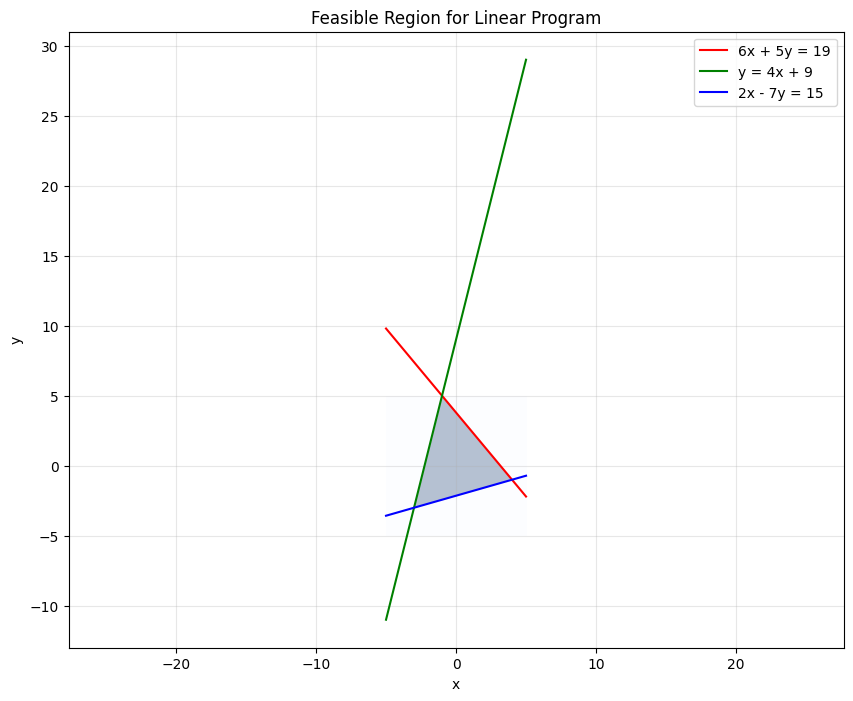
\includegraphics[width=0.75\textwidth]{plot.png}
    \caption{Feasible Region of the Linear Program}
    \label{fig:feasible_region}
\end{figure}

Using the naive approach, we need to compute the vertices of the feasible region. There are three lines, so we need to find the intersection of each pair of lines.

\begin{itemize}
\item Intersection of $6x + 5y = 19$ and $y = 4x + 9$:
\begin{align*}
6x + 5(4x + 9) &= 19 \\
26x + 45 &= 19 \\
26x &= -26 \\
x &= -1
\end{align*}
Therefore, $y = 4(-1) + 9 = 5$. So the intersection is $(-1, 5)$, and the value of the objective function is $-1 + 5 = 4$.

\item Intersection of $6x + 5y = 19 (e_1)$ and $2x - 7y = 15 (e_2)$:
Let $e_2 = 3e_2$, we get:
\begin{align*}
\left\{\begin{array}{l}
6x + 5y = 19 \\
6x - 21y = 45
\end{array}\right.
\end{align*}
Subtract the second equation from the first, we get:
\begin{align*}
26y = -26 \\
y = -1
\end{align*}
Substitute $y = -1$ into $e_1$, we get:
\begin{align*}
6x + 5(-1) = 19 \\
6x - 5 = 19 \\
6x = 24 \\
x = 4
\end{align*}
So the intersection is $(4, -1)$, and the value of the objective function is $4 + (-1) = 3$.

\item Intersection of $y = 4x + 9$ and $2x - 7y = 15$:
\begin{align*}
2x - 7(4x + 9) &= 15 \\
2x - 28x - 63 &= 15 \\
-26x &= 78 \\
x &= -3
\end{align*}
Substitute $x = -3$ into $y = 4x + 9$, we get:
\begin{align*}
y = 4(-3) + 9 = -12 + 9 = -3
\end{align*}
So the intersection is $(-3, -3)$, and the value of the objective function is $-3 + (-3) = -6$.

\end{itemize}

By comparing the values of the objective function at the vertices, we can see that the maximum value is $4$, which is attained at $(-1, 5)$. \\

Therefore, the maximum value of the objective function is $4$.

\newpage

\section*{Exercise 3}
\begin{enumerate}[(a)]
\item Rewrite the constraint $|x| + |y| \leq 5$ as a combination of linear constraints.
\item Show that there is no way to rewrite the constraint $|x| + |y| \geq 5$ as a combination of linear constraints.
\end{enumerate}

\textbf{Solution:}

(a) To rewrite $|x| + |y| \leq 5$ as linear constraints:

\begin{itemize}
\item $|x|$ can be either $x$ or $-x$ depending on whether $x$ is positive or negative. Similarly, $|y|$ can be either $y$ or $-y$.

\item This gives us four possible combinations:
   \begin{align*}
   \text{When } x \geq 0, y \geq 0: & \quad x + y \leq 5 \\
   \text{When } x \geq 0, y \leq 0: & \quad x - y \leq 5 \\
   \text{When } x \leq 0, y \geq 0: & \quad -x + y \leq 5 \\
   \text{When } x \leq 0, y \leq 0: & \quad -x - y \leq 5
   \end{align*}

\item Therefore, $|x| + |y| \leq 5$ is equivalent to the combination of the following linear constraints:
   \begin{align*}\left\{\begin{array}{l}
   x + y \leq 5 \\
   x - y \leq 5 \\
   -x + y \leq 5 \\
   -x - y \leq 5
   \end{array}\right.
   \end{align*}

\end{itemize}

(b) To prove that $|x| + |y| \geq 5$ cannot be written as a combination of linear constraints:

\begin{itemize}
\item Suppose, for contradiction, that $|x| + |y| \geq 5$ could be written as a combination of linear constraints.
\item The feasible region of $|x| + |y| \geq 5$ is the exterior of a diamond-shaped region(in this case, it is the union of the half-planes defined by the linear constraints, which is not necessarily convex), which is non-convex. We can verify this by taking two points (6, 0), and (-6, 0), which both satisfy $|x| + |y| = 6 > 5$, but the midpoint of the line segment connecting them does not, in this case, $|0| + |0| = 0 < 5$.
\item However, by definition of feasible region, it is the intersection of all half-planes defined by the linear constraints of the LP, which should be convex.
\item Contradiction.
\end{itemize}
Therefore, it is impossible to rewrite $|x| + |y| \geq 5$ as a combination of linear constraints.

\newpage

\section*{Exercise 4}
Consider the following LP:
\begin{align*}
\text{maximize} \quad & x_1 - 3x_2 - 2x_4 \\
x \in \mathbb{R}^4 \\
\text{subject to} \quad & \frac{1}{2}x_1 - \frac{7}{2}x_2 - \frac{3}{2}x_3 + \frac{7}{2}x_4 \leq 0, \\
& \frac{1}{2}x_1 - \frac{3}{2}x_2 - \frac{1}{2}x_3 + \frac{1}{2}x_4 \leq 0, \\
& x \geq 0
\end{align*}

\begin{enumerate}[(a)]
\item Perform two iterations of the simplex method using the following pivoting rule: choose the entering variable with the highest reduced cost. When both rows are valid leaving variables (in which case they'll always be tied for the smallest ratio) choose the basic variable for the first row as the leaving variable.
\item Comparing the resulting tableau to the original tableau, argue that the simplex method with this pivoting rule will cycle forever, returning to the same tableau every six steps.
\end{enumerate}

\textbf{Solution: } \\

(a) Two iterations of the simplex method with the given pivot rule.\\

Step 1: Construct the initial tableau. \\

We take the basic variables to be \(s_1, s_2\) initially (each slack variable corresponding to one row), and treat \(x_1, x_2, x_3, x_4\) as nonbasic.  We also introduce the objective row in the form
\[
z \;-\; x_1 \;+\; 3\,x_2 \;+\; 2\,x_4 \;=\; 0.
\]
Therefore, we can construct the initial tableau as follows:

\[
\begin{array}{c|cccccc|c}
  & x_1 & x_2 & x_3 & x_4 & s_1 & s_2 & \text{RHS}\\\hline
s_1 & \tfrac12 & -\tfrac72 & -\tfrac32 & \tfrac72 & 1 & 0 & 0\\
s_2 & \tfrac12 & -\tfrac32 & -\tfrac12 & \tfrac12 & 0 & 1 & 0\\\hline
-z   & -1       & 3         & 0         & 2        & 0 & 0 & 0
\end{array}
\]

Step 2: Determine the entering variable. \\

We are doing a \emph{maximization} problem, so in the objective row (the \(z\)-row) we look for the largest (most positive) coefficient among the nonbasics, which is \(3\) (for \(x_2\)).  However, looking at the entry value, both $-\frac{7}{2}$ and $-\frac{3}{2}$ are negative, so we need to find the other reduced cost, which is 2 (for \(x_4\)).  Therefore, \(x_4\) enters the basis.

Step 3: Determine the leaving variable (ratio test). \\

We look only at rows where the pivot column's coefficient is \(\ge 0\).  In row~\(s_1\) and ~\(s_2\), the \(x_4\)-coefficient is \(\,\tfrac72\) and \(\,\tfrac12\) respectively, which is \emph{positive}.  However, since the RHS are both 0, the ratios are both 0 as well. According to the rule, we need to choose the first row's basic variable to leave, which is \(s_1\). \\

Step 4: Pivot. \\

We now pivot on the entry in the \(x_4\)-column and the \(s_1\)-row.  This gives us the new tableau:

\[
\begin{array}{c|cccccc|c}
  & x_1 & x_2 & x_3 & x_4 & s_1 & s_2 & \text{RHS}\\\hline
s_1 & \tfrac17 & -1 & -\tfrac37 & 1 & \tfrac27 & 0 & 0\\
s_2 & \tfrac37 & -1 & -\tfrac27 & 0 & -\tfrac17 & 1 & 0\\\hline
-z   & -\tfrac97       & 5         & \tfrac{6}{7}         & 0        & -\tfrac{4}{7} & 0 & 0
\end{array}
\]

Step 5: Determine the entering variable. \\

We are doing a \emph{maximization} problem, so in the objective row (the \(z\)-row) we look for the largest (most positive) coefficient among the nonbasics, which is \(3\) (for \(x_2\)).  However, looking at the entry value, both $-\frac{7}{2}$ and $-\frac{3}{2}$ are negative, so we need to find the other reduced cost, which is 2 (for \(x_4\)).  Therefore, \(x_4\) enters the basis.

\newpage

\section*{Exercise 5}
Consider an LP of the form
\begin{align*}
\text{maximize} \quad & c^\top x \\
x \in \mathbb{R}^n \\
\text{subject to} \quad & Ax \leq b
\end{align*}

Let $u, v \in \mathbb{R}^n$ be feasible solutions. Prove that $u$ and $v$ are optimal solutions if and only if $(u + v)/2$ is an optimal solution. \\

\textbf{Solution: } \\

Since this is a if and only if statement, we need to prove both directions. \\

($\Rightarrow$) First, let's prove that if $u$ and $v$ are optimal solutions, then $(u + v)/2$ is an optimal solution.

1) Since $u$ and $v$ are feasible solutions:
   \[ Au \leq b \text{ and } Av \leq b \]

2) Therefore:
   \[ A(\frac{u + v}{2}) = \frac{Au + Av}{2} \leq \frac{b + b}{2} = b \]
   Thus, $(u + v)/2$ is feasible.

3) Since $u$ and $v$ are optimal solutions, they achieve the same objective value:
   \[ c^\top u = c^\top v = z^* \]
   where $z^*$ is the optimal objective value.

4) Therefore:
   \[ c^\top(\frac{u + v}{2}) = \frac{c^\top u + c^\top v}{2} = \frac{z^* + z^*}{2} = z^* \]

5) Hence, $(u + v)/2$ achieves the optimal objective value and is feasible, making it an optimal solution. \\

($\Leftarrow$) Now, let's prove that if $(u + v)/2$ is optimal, then both $u$ and $v$ are optimal. \\

1) Let $z^*$ be the optimal objective value. Then:
   \[ c^\top(\frac{u + v}{2}) = z^* \]

2) By linearity:
   \[ \frac{c^\top u + c^\top v}{2} = z^* \]

3) Since $u$ and $v$ are feasible solutions:
   \[ c^\top u \leq z^* \text{ and } c^\top v \leq z^* \]

4) If either $c^\top u < z^*$ or $c^\top v < z^*$, then:
   \[ \frac{c^\top u + c^\top v}{2} < z^* \]
   This would contradict step 2.

5) Therefore:
   \[ c^\top u = z^* \text{ and } c^\top v = z^* \]

Thus, both $u$ and $v$ must be optimal solutions. \\

\textbf{Conclusion:} We have shown both directions of the if and only if statement, completing the proof.

\end{document}